\documentclass[aspectratio=169,11pt]{beamer}
\usepackage[T1]{fontenc}
\usepackage{lmodern,amsmath,amssymb,mathtools,bm,booktabs,array,graphicx,tikz}
\usetikzlibrary{arrows.meta,positioning,calc,decorations.pathreplacing,patterns}
\definecolor{ink}{HTML}{17344D}\definecolor{accent}{HTML}{087E8B}\definecolor{pale}{HTML}{EDF5F5}\definecolor{gold}{HTML}{AD6B19}
\providecommand{\dd}{\,\mathrm{d}}\providecommand{\R}{\mathbb{R}}
\providecommand{\E}{\mathbb{E}}\providecommand{\Var}{\operatorname{Var}}
\providecommand{\Cov}{\operatorname{Cov}}\providecommand{\diag}{\operatorname{diag}}
\providecommand{\norm}[1]{\left\lVert#1\right\rVert}
\providecommand{\abs}[1]{\left|#1\right|}
\usefonttheme{professionalfonts}
\setbeamercolor{normal text}{fg=black,bg=white}
\setbeamercolor{frametitle}{fg=ink,bg=white}
\setbeamercolor{title}{fg=ink}\setbeamercolor{structure}{fg=accent}
\setbeamercolor{block title}{fg=ink,bg=pale}\setbeamercolor{block body}{fg=black,bg=pale!40}
\setbeamercolor{alerted text}{fg=accent}
\setbeamerfont{frametitle}{size=\Large,series=\bfseries}
\setbeamerfont{title}{size=\LARGE,series=\bfseries}
\setbeamertemplate{navigation symbols}{}
\setbeamersize{text margin left=.7cm,text margin right=.7cm}
\setbeamertemplate{frametitle}{\vspace{.18cm}\insertframetitle\par\vspace{.1cm}{\color{accent}\hrule height .6pt}\vspace{.12cm}}
\newcommand{\notestarget}{notes.pdf}\newcommand{\noteslabel}{Notes}
\setbeamertemplate{footline}{\hspace{.7cm}\color{ink}\scriptsize Computational Cardiology\quad\href{\notestarget}{\noteslabel}\hfill\insertframenumber\,/\,\inserttotalframenumber\hspace{.7cm}\vspace{.18cm}}
\setbeamercovered{invisible}
\hypersetup{pdfauthor={Zan Ahmad},pdftitle={Finite-volume advection and diffusion},pdfpagemode=UseNone}
\begin{document}
\begin{frame}[plain]\vfill
{\small\color{accent} Computational Cardiology \quad Lecture 5}\par\medskip
{\raggedright\hyphenpenalty=10000\exhyphenpenalty=10000\LARGE\bfseries\color{ink} Finite-volume advection and diffusion}\par\bigskip
Zan Ahmad\par\smallskip
{\small Fall 2024}\par\vfill\end{frame}
\renewcommand{\notestarget}{notes.pdf\#note-control-volumes-and-the-boundary-budget}
\begin{frame}[t,fragile,label=slide-the-represented-concentration]{The represented concentration}
\[\bar c_i=\frac1{\Delta x}\int_{x_{i-1/2}}^{x_{i+1/2}}c(x,t)\,\mathrm dx.\]\pause{} The unknown is a cell average, not a value at an arbitrary point.
\end{frame}
\renewcommand{\notestarget}{notes.pdf\#note-control-volumes-and-the-boundary-budget}
\begin{frame}[t,fragile,label=slide-integrate-the-conservation-law]{Integrate the conservation law}
\[c_t+J_x=0\quad\Longrightarrow\quad\Delta x\,\dot{\bar c}_i=J_{i-1/2}-J_{i+1/2}.\]\pause{} The same face flux enters adjacent cells with opposite signs.
\end{frame}
\renewcommand{\notestarget}{notes.pdf\#note-control-volumes-and-the-boundary-budget}
\begin{frame}[t,fragile,label=slide-the-global-boundary-budget]{The global boundary budget}
\[M=\Delta x\sum_i c_i,\qquad M^{n+1}-M^n=\Delta t(J_{1/2}-J_{N+1/2}).\]\pause{} Periodic endpoints have identical fluxes.
\end{frame}
\renewcommand{\notestarget}{notes.pdf\#note-advective-and-diffusive-fluxes}
\begin{frame}[label=slide-constitutive-transport-flux-figure]{Transport redistributes a conserved amount}
\centering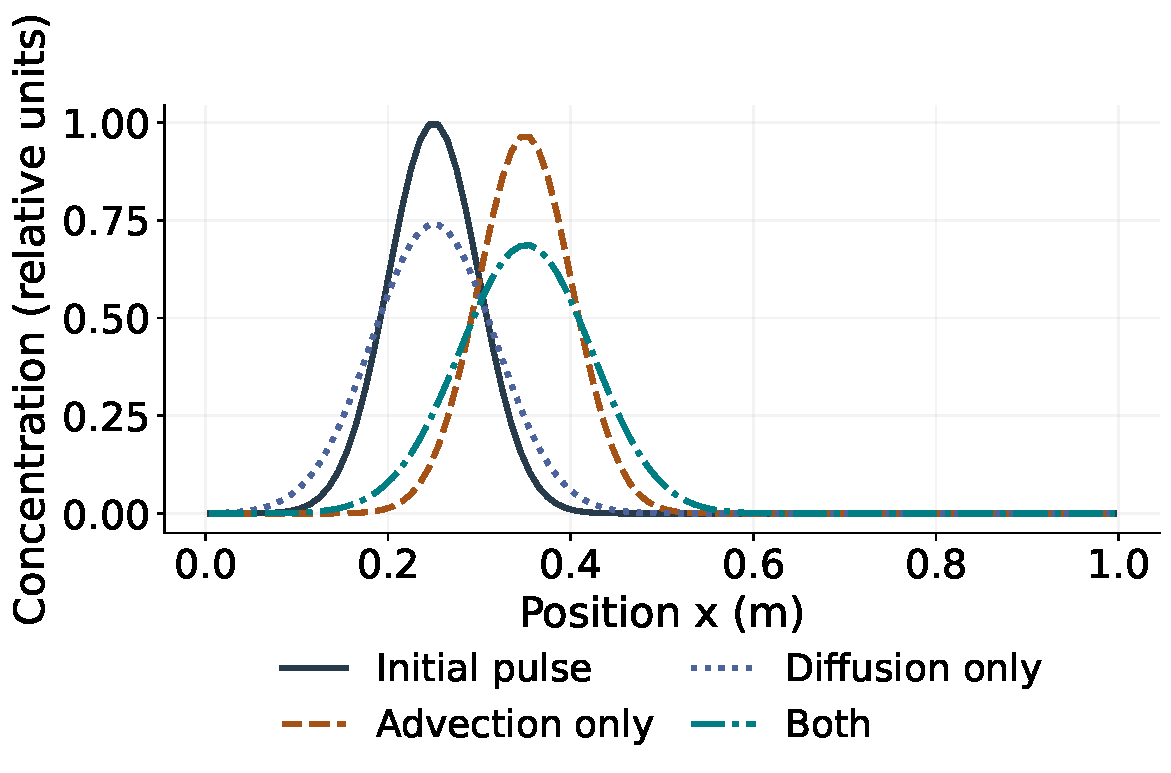
\includegraphics[width=.98\linewidth,height=.69\textheight,keepaspectratio]{presentation-figures/transport-pulse-panel-1.pdf}\end{frame}
\renewcommand{\notestarget}{notes.pdf\#note-advective-and-diffusive-fluxes}
\begin{frame}[t,fragile,label=slide-constitutive-transport-flux]{Constitutive transport flux}
\[J=ac-Dc_x,\qquad [a]=\mathrm{m/s},\quad[D]=\mathrm{m^2/s}.\]\pause{}\[c_t=-ac_x+Dc_{xx}.\]
\end{frame}
\renewcommand{\notestarget}{notes.pdf\#note-the-upwind-stencil-and-a-discrete-maximum-principle}
\begin{frame}[t,fragile,label=slide-upwind-advection]{Upwind advection}
\[a^+=\max(a,0),\quad a^-=\min(a,0).\]\pause{}\[J_{i+1/2}^{\rm adv}=a^+c_i+a^-c_{i+1}.\] The upstream cell changes when the velocity changes sign.
\end{frame}
\renewcommand{\notestarget}{notes.pdf\#note-the-upwind-stencil-and-a-discrete-maximum-principle}
\begin{frame}[t,fragile,label=slide-centered-diffusion]{Centered diffusion}
\[J_{i+1/2}^{\rm diff}=-D\frac{c_{i+1}-c_i}{\Delta x}.\]\pause{} A concentration increasing to the right produces a diffusive flux to the left.
\end{frame}
\renewcommand{\notestarget}{notes.pdf\#note-the-upwind-stencil-and-a-discrete-maximum-principle}
\begin{frame}[t,fragile,label=slide-the-positive-velocity-update]{The positive-velocity update}
\[c_i^{n+1}=(\nu+\mu)c_{i-1}^n+(1-\nu-2\mu)c_i^n+\mu c_{i+1}^n.\]\pause{}\[\nu=\frac{a\Delta t}{\Delta x},\qquad\mu=\frac{D\Delta t}{\Delta x^2}.\]
\end{frame}
\renewcommand{\notestarget}{notes.pdf\#note-the-upwind-stencil-and-a-discrete-maximum-principle}
\begin{frame}[t,fragile,label=slide-a-discrete-maximum-principle]{A discrete maximum principle}
If $\nu+2\mu\le1$, all three coefficients are nonnegative and sum to one.\pause{}\[\min_jc_j^n\le c_i^{n+1}\le\max_jc_j^n.\]
\end{frame}
\renewcommand{\notestarget}{notes.pdf\#note-the-upwind-stencil-and-a-discrete-maximum-principle}
\begin{frame}[t,fragile,label=slide-a-time-step-restriction-for-either-direction]{A time-step restriction for either direction}
\[\Delta t\left(\frac{|a|}{\Delta x}+\frac{2D}{\Delta x^2}\right)\le1.\]\pause{} Halving $\Delta x$ doubles the advective rate and quadruples the diffusive rate.
\end{frame}
\renewcommand{\notestarget}{notes.pdf\#note-an-open-boundary-calculation}
\begin{frame}[label=slide-an-open-boundary-step-panel-1]{Internal transfers cancel}
\centering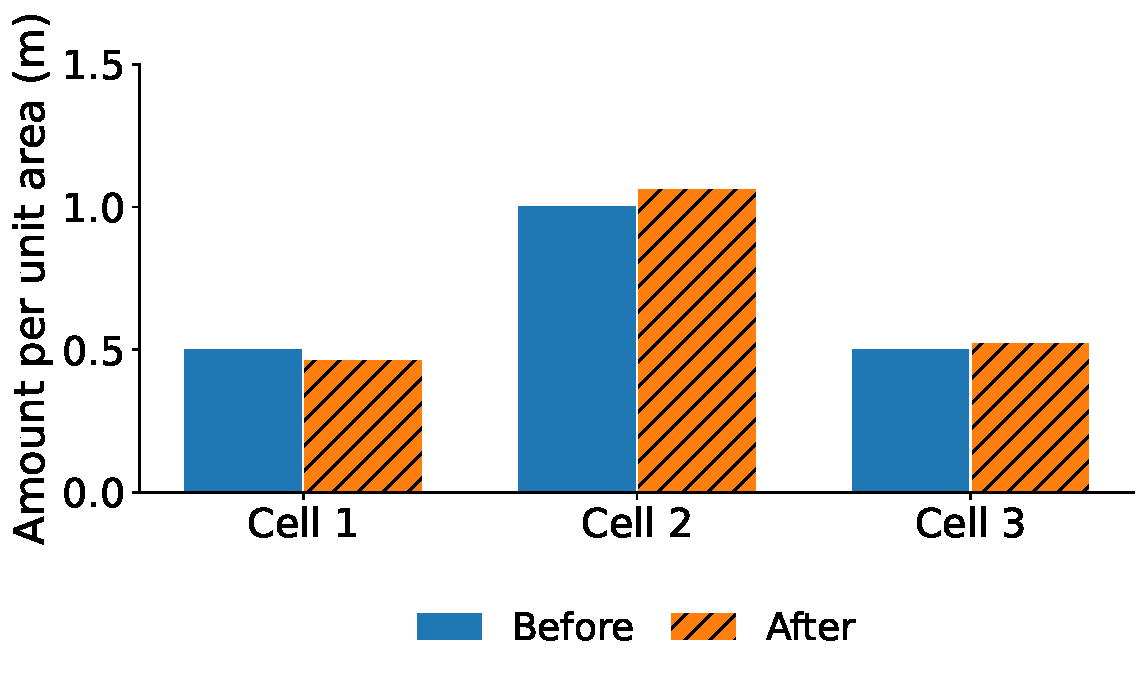
\includegraphics[width=.98\linewidth,height=.69\textheight,keepaspectratio]{presentation-figures/flux-budget-panel-1.pdf}\end{frame}
\renewcommand{\notestarget}{notes.pdf\#note-an-open-boundary-calculation}
\begin{frame}[label=slide-an-open-boundary-step-panel-2]{Boundary flux sets the change}
\centering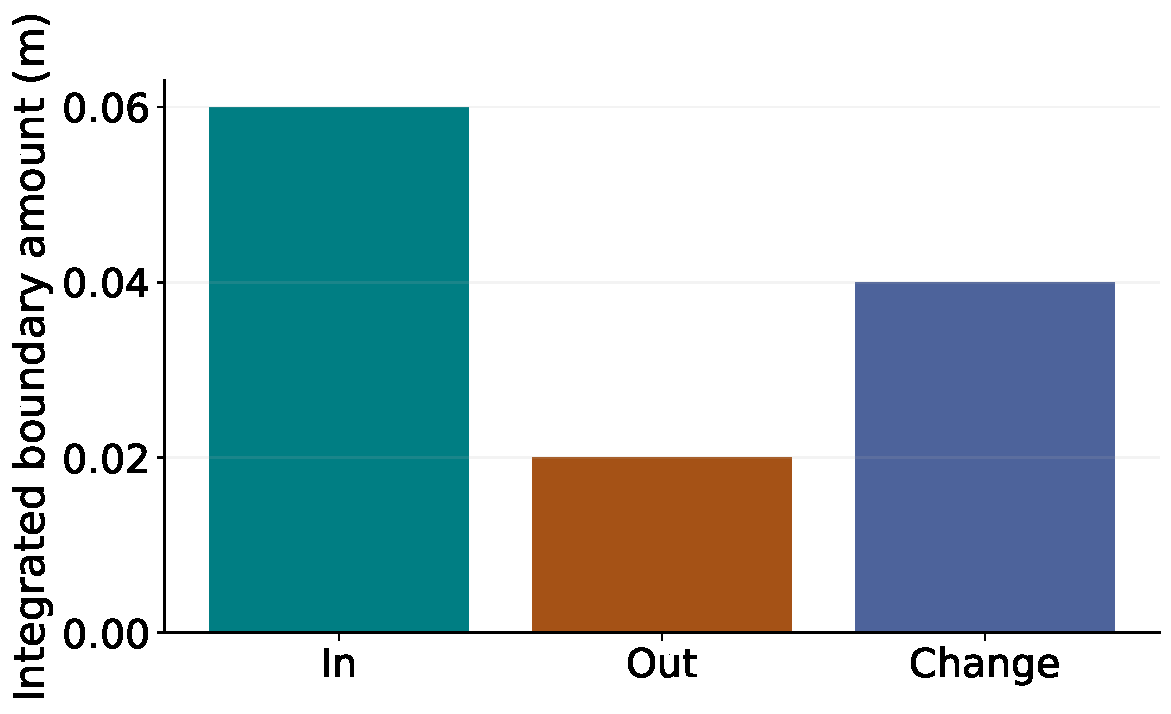
\includegraphics[width=.98\linewidth,height=.69\textheight,keepaspectratio]{presentation-figures/flux-budget-panel-2.pdf}\end{frame}
\renewcommand{\notestarget}{notes.pdf\#note-an-open-boundary-calculation}
\begin{frame}[t,fragile,label=slide-an-open-boundary-step]{An open-boundary step}
\[c^n=(1,2,1),\quad \Delta x=.5,\quad\Delta t=.2.\]\pause{} Four prescribed face fluxes $(.3,.5,.2,.1)$ give $c^{n+1}=(.92,2.12,1.04)$.
\end{frame}
\renewcommand{\notestarget}{notes.pdf\#note-an-open-boundary-calculation}
\begin{frame}[t,fragile,label=slide-the-amount-balance]{The amount balance}
\[M^n=2,\qquad M^{n+1}=2.04.\]\pause{}\[\Delta M=.2(.3-.1)=.04.\] Internal faces redistribute amount without changing this total.
\end{frame}
\renewcommand{\notestarget}{notes.pdf\#note-periodic-transport-and-limiting-cases}
\begin{frame}[t,fragile,label=slide-an-exact-shift-of-the-cell-vector]{An exact shift of the cell vector}
For $D=0$ and $\nu=1$,\[c_i^{n+1}=c_{i-1}^n.\]\pause{} Negative velocity reverses the shift. This identity fixes the indexing convention.
\end{frame}
\renewcommand{\notestarget}{notes.pdf\#note-periodic-transport-and-limiting-cases}
\begin{frame}[t,fragile,label=slide-constant-and-stationary-states]{Constant and stationary states}
If $c_i=c_0$, every flux difference is zero.\pause{} If $a=D=0$, every cell is unchanged, including nonconstant states.
\end{frame}
\renewcommand{\notestarget}{notes.pdf\#note-physical-and-numerical-diffusion}
\begin{frame}[t,fragile,label=slide-numerical-diffusion]{Numerical diffusion}
For smooth pure advection with $a>0$, the leading modified equation is\[c_t+ac_x=\frac{a\Delta x}{2}(1-\nu)c_{xx}+\cdots.\]\pause{} Upwind smoothing can occur even when the physical $D$ is zero.
\end{frame}
\renewcommand{\notestarget}{notes.pdf\#note-physical-and-numerical-diffusion}
\begin{frame}[t,fragile,label=slide-transport-mechanisms-and-model-interpretation]{Transport mechanisms and model interpretation}
A tracer requires a justified velocity field and inlet conditions. An activation model requires reaction kinetics.\pause{} The same balance structure can support these models, but the scalar pulse does not supply their missing physics.
\end{frame}
\end{document}
